\documentclass[11pt,addpoints,answers]{exam}

%%%%%%%%%%%%%%%%%%%%%%%%%%%%%%%%%%%%%%%%%%%%%%%%%%%%%%%%5
% Packages
%%%%%%%%%%%%%%%%%%%%%%%%%%%%%%%%%%%%%%%%%%%%%%%%%%%%%%%%5
\usepackage{amssymb,amsmath,amsthm,amsfonts,mathtools,dsfont,thmtools}
\usepackage{suffix}
\usepackage{natbib} 
\usepackage{csquotes} 
\usepackage{subcaption}
\usepackage[inline]{enumitem} 
\usepackage{booktabs}
\usepackage[usenames,dvipsnames]{xcolor}
\usepackage[breakable]{tcolorbox} 
\usepackage{wrapfig}

\usepackage{tikz}
\usepackage{tikz-qtree}
\usetikzlibrary{bayesnet}
\usepackage{hyperref}
\usepackage[capitalize,noabbrev]{cleveref}

%%%%%%%%%%%%%%%%%%%%%%%%%%%%%%%%%%%%%%%%%%%%%%%%%%%%%%%%5
% Formatting
%%%%%%%%%%%%%%%%%%%%%%%%%%%%%%%%%%%%%%%%%%%%%%%%%%%%%%%%5

\hypersetup{
  colorlinks=true,
  linkcolor=RawSienna,
  urlcolor=Cyan,
  citecolor=gray
}

\setlength{\parskip}{6pt}
\setlength{\parindent}{0pt}
\setlength{\headheight}{14pt}

% Custom Shortcuts
\usepackage{listings}
\usepackage{adjustbox}
\usepackage{tikz}
\usetikzlibrary{arrows.meta,positioning}
\usepackage{algorithm}
\usepackage{algcompatible}

\chead{EN.601.475/675 Machine Learning}
\date{}
\pagestyle{headandfoot}
\begin{document}
\thispagestyle{headandfoot}

\begin{center}
  {\Large \bf{Homework 3: Due \textbf{Wednesday, October 15th, 11:59pm}}}
\end{center}

\qformat{\textbf{\Large Question \thequestion\ \dotfill \emph{\totalpoints\ points}}}

\begin{center}
\fbox{\fbox{\parbox{6.5in}{
\textbf{Submission Instructions:} You will upload your solutions to the analytical portion and the programming portion separately to Gradescope.  
\begin{itemize}
\item \textbf{Analytical Part (this file)}: You should use LaTeX to type up your solutions (e.g., via Overleaf or similar), but please ensure that \textbf{each part (e.g., a, b, etc) begins on a new page} (to facilitate grading in Gradescope). You will upload the PDF to the assignment ``Homework 3: Analytical'' on Gradescope.
\item \textbf{Programming Part (see Canvas)}: You should upload your \texttt{.ipynb} file directly to Gradescope under the assignment ``Homework 3: Programming''.
\end{itemize}
Note that you must upload \textbf{both} parts to their respective assignments on Gradescope.
\vspace{0.1in}

\textbf{Collaboration Policy:} You may work with other students on the homework assignments, but you must write up and submit your own work independently, and you must acknowledge your collaborators on the first page of your homework submission.
\vspace{0.1in}

\textbf{Late Submission Policy:} You have up to 48 hours of ``slack'' for late submissions of homework assignments, across \textbf{all} homework assignments.  Once you have exhausted your budget, we will deduct points for late submissions.  However, \textbf{no individual assignment may be submitted more than 48 hours late}, as we will release solutions at this time.
\vspace{0.1in}

\textbf{Use of Generative AI:} You are \textbf{not permitted} to use generative AI tools (e.g., ChatGPT) for problems on this problem set.
}}}
\end{center}

% TODO: Type out your name and email in these spaces, replacing the \enspace\hrulefill
\makebox[\textwidth]{Name:\enspace Rashed Aldulijan}\vspace{0.2in}
\makebox[\textwidth]{JHU Email:\enspace ralduli1@jk.edu}\vspace{0.2in}
\makebox[\textwidth]{Collaborators (or \enquote{None}):\enspace None}

\begin{center}
The analytical portion (this file) has \numquestions\ questions, for a total of \numpoints\
points.
\end{center}

\newpage

\section*{Part 1: Analytical Questions}

\begin{questions}
\question%
In this question, we will apply the algorithm used to train AdaBoost on a binary classification problem with ``decision stumps'' (single split decision trees) as weak learners. The labels are $y \in \{+1,-1\}$.
The three decision stumps we will use are defined as follows, using the indicator notation:
\[
h_1(x) = \mathbf{1}\{\texttt{free}=1\}, \quad
h_2(x) = \mathbf{1}\{\texttt{money}=1\}, \quad
h_3(x) = \mathbf{1}\{\texttt{win}=1\},
\]
where (for the purposes of this problem) $\mathbf{1}\{\cdot\}$ returns $+1$ if the condition is true and $-1$ otherwise.  
We have the following dataset of $n=8$ emails, where the columns represent specific words found in an email, and the $+1$ label represents ``spam,'' $-1$ label represents ``not spam'':

\[
\begin{array}{c|c|c|c|c}
i & \texttt{free} & \texttt{money} & \texttt{win} & y \\
\hline
1 & 1 & 0 & 0 & +1 \\
2 & 0 & 1 & 0 & +1 \\
3 & 0 & 0 & 1 & -1 \\
4 & 1 & 1 & 0 & +1 \\
5 & 0 & 0 & 0 & -1 \\
6 & 0 & 1 & 1 & +1 \\
7 & 1 & 0 & 1 & +1 \\
8 & 0 & 0 & 1 & +1 \\
\end{array}
\]

Weights initialize as $D_1(i)=1/8$.  
Recall that at round $t$ we have:
\[
\varepsilon_t = \Pr_{i \sim D_t}[h_t(x_i)\neq y_i], \quad
\alpha_t = \tfrac12 \ln \frac{1-\varepsilon_t}{\varepsilon_t} \quad
D_{t+1}(i) \propto D_t(i) \exp(-\alpha_t y_i h_t(x_i)).
\]

\begin{parts}
\part[5]%
 For each weak learner $h_j$, compute $\varepsilon_1(h_j) = \Pr_{i \sim D_1}[h_j(x_i) \neq y_i]$.  Which of the three is the best weak learner? Using the best weak learner, compute $\alpha_1$ and $D_2$.
\begin{solutionorbox}  
  First, compute the error rates for each weak learner:
  \[
  \varepsilon_1(h_1) = \Pr_{i \sim D_1}[h_1(x_i) \neq y_i] = \frac{2}{8} = 0.375,
  \]
  \[
  \varepsilon_1(h_2) = \Pr_{i \sim D_1}[h_2(x_i) \neq y_i] = \frac{1}{8} = 0.375,
  \]
  \[
  \varepsilon_1(h_3) = \Pr_{i \sim D_1}[h_3(x_i) \neq y_i] = \frac{3}{8} = 0.5.
  \]
  Both $h_1$ and $h_2$ have the lowest error rate of 0.375. We can choose either as the best weak learner. Let's choose $h_1$.
  \[
  \alpha_1 = \frac{1}{2} \ln \frac{1 - 0.375}{0.375} = \frac{1}{2} \ln \frac{0.625}{0.375} = \frac{1}{2} \ln \frac{5}{3} \approx 0.2554.
  \]
  Let's compute $D_2(i)$ for each $i$:
  \[
  D_2(i) \propto 1/8 \cdot \exp(-\alpha_1) = 0.09.
  \]
  where i is classified correctly by $h_1$ (i.e., $i=1,3,4,5,7$).
  \[
  D_2(i) \propto 1/8 \cdot \exp(\alpha_1) = 0.1613.
  \]
  where i is misclassified by $h_1$ (i.e., $i=2,6,8$).
  
   
\end{solutionorbox}

\newpage
\part[5]%
Explain how AdaBoost’s reweighting helps when rare positive (+1) emails are initially misclassified by obvious word stumps like h1 (free).
\begin{solutionorbox}
  In this example, we had weight of 0.1613 for the misclassified spam emails, which is higher than the initial weight of 0.125. This increase in weight means that in the next round of boosting, the algorithm will pay more attention to these misclassified positive emails. As a result, it is more likely to select a weak learner that can correctly classify these rare positive emails, which improves the overall performance of the ensemble model.
\end{solutionorbox}

\newpage
\part[5]%
Explain how AdaBoost can incorporate a learner that does worse than random, in other words a learner for which  $\varepsilon_t > 0.5$.
\begin{solutionorbox}
  \[
  H_t(x) = \text{sign}\left(\sum_{s=1}^t \alpha_s h_s(x)\right).
  \]
  If a weak learner $h_t$ has an error rate $\varepsilon_t > 0.5$, which means $\alpha_t$ is small. AdaBoost incorporate these weak learner but it gives it smaller $\alpha$ as the error get larger, so it has less influence on the final prediction. This way, AdaBoost can still benefit from the weak learner's contribution, even if it performs worse than random guessing.
\end{solutionorbox}
\end{parts}

\newpage
\question%
Consider the following mini convolutional neural net, where $(x_1, x_2, x_3)$ is the input, followed by a convolution layer with a filter $(w_1, w_2)$, a ReLU layer, and a fully connected layer with weight $(v_1, v_2)$. 

\begin{center}
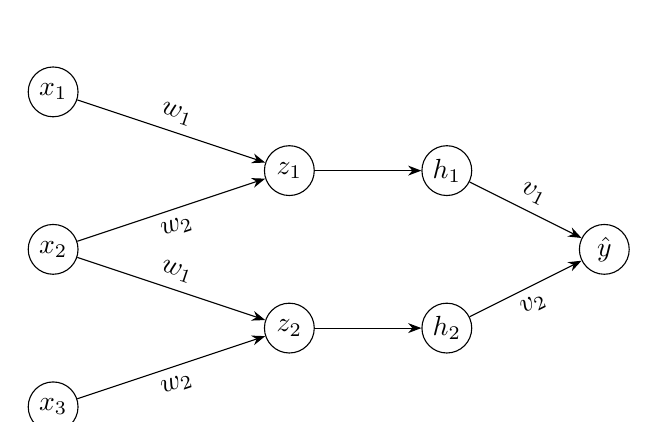
\begin{tikzpicture}[
    >=Stealth,
    node/.style={circle,draw,minimum size=18pt,inner sep=0pt},
    every edge quotes/.style = {auto, text=black, font=\normalsize}
]
\node[node] (x1)   at (-4,  2) {$x_1$};
\node[node] (x2)   at (-4,  0) {$x_2$};
\node[node] (x3)   at (-4, -2) {$x_3$};

\node[node] (a1)   at (-1,  1) {$z_1$};
\node[node] (a2)   at (-1, -1) {$z_2$};

\node[node] (z1)   at ( 1,  1) {$h_1$};
\node[node] (z2)   at ( 1, -1) {$h_2$};

\node[node] (yhat) at ( 3,  0) {$\hat{y}$};

\draw[->] (x1) -- (a1) node[midway,sloped,above] {$w_1$};
\draw[->] (x2) -- (a1) node[midway,sloped,below] {$w_2$};

\draw[->] (x2) -- (a2) node[midway,sloped,above] {$w_1$};
\draw[->] (x3) -- (a2) node[midway,sloped,below] {$w_2$};

\draw[->] (a1) -- (z1);
\draw[->] (a2) -- (z2);

\draw[->] (z1) -- (yhat) node[midway,sloped,above] {$v_1$};
\draw[->] (z2) -- (yhat) node[midway,sloped,below] {$v_2$};
\end{tikzpicture}
\end{center}

More concretely, the computation is specified by
\[
z_1 = x_1w_1 + x_2w_2, \quad 
z_2 = x_2w_1 + x_3w_2,
\]
\[
h_1 = \max\{0,z_1\}, \quad 
h_2 = \max\{0,z_2\},
\]
\[
\hat{y} = h_1 v_1 + h_2 v_2.
\]

We assume the true labels $y$ are $-1$ or $1$, so that $(x,y) \in \mathbb{R}^3 \times \{-1,+1\}$. 

The logistic loss CNN can then be written as follows
\[
\ell(y, \hat{y}) = \ln(1 + \exp(-y\hat{y})),
\]
which is a function of the parameters of the network: $w_1, w_2, v_1, v_2$.

\begin{parts}
\part[5]%
Write down $\frac{\partial \ell}{\partial v_1}$ and $\frac{\partial \ell}{\partial v_2}$ (show the intermediate steps that use chain rule). You can use the sigmoid function $\sigma(z) = \frac{1}{1+e^{-z}}$ to simplify your notation.

\begin{solutionorbox}[3.5in]
  \[
  \frac{\partial \ell}{\partial \hat{y}} = -\frac{y}{1 + e^{y\hat{y}}} = -y \sigma(-y\hat{y}).
  \]
  \[ \frac{\partial \hat{y}}{\partial v_1} = h_1, \quad \frac{\partial \hat{y}}{\partial v_2} = h_2. \]
  \[
\frac{\partial \ell}{\partial v_1} = \frac{\partial \ell}{\partial \hat{y}} \cdot \frac{\partial \hat{y}}{\partial v_1} = \boxed{-y \sigma(-y\hat{y}) h_1},
  \]
  \[
  \frac{\partial \ell}{\partial v_2} = \frac{\partial \ell}{\partial \hat{y}} \cdot \frac{\partial \hat{y}}{\partial v_2} = \boxed{-y \sigma(-y\hat{y}) h_2}.
  \]
\end{solutionorbox}

\newpage
\part[5]%
Write down $\frac{\partial \ell}{\partial w_1}$ and $\tfrac{\partial \ell}{\partial w_2}$ (show the intermediate steps that use chain rule). The derivative of the ReLU function is $H(a) = \mathbf{1}[a > 0]$, which you can use directly in your answer. In particular (by convention), we take the gradient of the ReLU function to be zero when $a = 0$.\footnote{While the ReLU function is not differentiable at $a = 0$, zero is a \textit{subgradient}, a generalization of the gradient to convex non-differentiable functions.}

\begin{solutionorbox}[3.5in]
  \[
  \frac{\partial \ell}{\partial w_1} = \frac{\partial \ell}{\partial \hat{y}} \cdot \left( \frac{\partial \hat{y}}{\partial h_1} \cdot \frac{\partial h_1}{\partial z_1} \cdot \frac{\partial z_1}{\partial w_1} + \frac{\partial \hat{y}}{\partial h_2} \cdot \frac{\partial h_2}{\partial z_2} \cdot \frac{\partial z_2}{\partial w_1} \right).
  \]
  We already have $\frac{\partial \ell}{\partial \hat{y}} = -y \sigma(-y\hat{y})$.
  \[
  \frac{\partial \hat{y}}{\partial h_1} = v_1, \quad \frac{\partial h_1}{\partial z_1} = H(z_1), \quad \frac{\partial z_1}{\partial w_1} = x_1,
  \]
  \[
  \frac{\partial \hat{y}}{\partial h_2} = v_2, \quad \frac{\partial h_2}{\partial z_2} = H(z_2), \quad \frac{\partial z_2}{\partial w_1} = x_2.
  \]
  \[
  \frac{\partial \ell}{\partial w_1} = -y\sigma(-y\hat{y}) (v_1 H(z_1) x_1 + v_2 H(z_2) x_2) = \boxed{-y\sigma(-y\hat{y}) (v_1 H(z_1) x_1 + v_2 H(z_2) x_2)}.
  \]
  
  Similarly,
  \[
  \frac{\partial \ell}{\partial w_2} = -y\sigma(-y\hat{y}) (v_1 H(z_1) x_2 + v_2 H(z_2) x_3) = \boxed{-y\sigma(-y\hat{y}) (v_1 H(z_1) x _2 + v_2 H(z_2) x_3)}.
  \]
\end{solutionorbox}

\newpage
\part[3]%
We often initialize the weights of neural networks randomly. Suppose we ignored this practice, and instead we initialized all of the parameters $v_1, v_2, w_1, w_2$ as zero. What is the value of $z_1, z_2, h_1, h_2, \hat{y}$ with this initialization?  What happens to the gradient in this case?  In conclusion, why is this a poor choice of initialization?

\begin{solutionorbox}
  all gradients are zero, the weights will not be updated during training. $\hat{y}$ will be zero, and the loss will always be 2. This means the model will not learn from the data, making this a poor choice of initialization.
\end{solutionorbox}

\newpage
\part[2]%
Using the derivations above, fill in the missing details of the backpropagation algorithm below that is used to train this mini CNN.

\begin{algorithm}[H]
\caption{Backpropagation for the above mini CNN}
\begin{algorithmic}
\State \textbf{Input:} A training set $(x_1,y_1), \dots, (x_n,y_n)$
\State \textbf{Initialize:} set $w_1,w_2,v_1,v_2$ randomly
  \State Randomly pick an example $(x_i,y_i)$

  \State Forward propagation:
  
\begin{solutionorbox}[4in]
  \textbf{compute}
  \[
  z_1 = x_1w_1 + x_2 w_2, \quad 
  z_2 = x_2 w_1 + x_3 w_2,
  \]
  \[
  h_1 = \max(0, z_1), \quad 
  h_2 = \max(0, z_2), \quad
  \hat{y} = v_1 h_1 + v_2 h_2
  \]
\end{solutionorbox}

  \State Backward propagation:
\begin{solutionorbox}[4in]
  
  \textbf{compute}
  \[
  g_{w_1} = -y\sigma(-y\hat{y}) (v_1 H(z_1) x_1 + v_2 H(z_2) x_2),
  \]
  \[
  g_{w_2} = -y\sigma(-y\hat{y}) (v_1 H(z_1) x_2 + v_2 H(z_2) x_3),
  \]
  \[
  g_{v_1} = -y\sigma(-y\hat{y}) h_1,
  \qquad
  g_{v_2} = -y\sigma(-y\hat{y}) h_2.
  \]

  \textbf{Output:} \
  return $g_{w_1}, g_{w_2}, g_{v_1}, g_{v_2}$ 
\end{solutionorbox}
\end{algorithmic}
\end{algorithm}

\end{parts}

\newpage
\question%
{\bf Dropout Regularization and Variance}

One approach to regularization in a neural network model is dropout. During training, dropout is applied independently to each unit (either inputs $x_i$, or hidden units $h_{li}$), setting them to zero with probability $p$, and otherwise scaling them by $1 / (1 - p)$. This is only applied during model training: during final model evaluation, the units are unchanged.

\begin{parts}
\part[5]
We will consider a simple linear model $\hat{y} = w^\top x$, with dropout applied to the inputs $x$.  To start, derive the expectation and covariance matrix of the effective input vector $\tilde{x}$ when dropout is applied. Treat the inputs $x$ as fixed, so that dropout is the only source of randomness (and hence the only source of randomness to consider in computing expectation and covariance).

\begin{solutionorbox}
\end{solutionorbox}

\newpage
\part[7]%
Again, treating the data $y, x$ and the weights $w$ as fixed, show that the expected squared loss under dropout (i.e., during training) can be written as the original squared loss plus an extra penalty on the weights. 

\begin{solutionorbox}
\end{solutionorbox}

\newpage
\part[3]
Interpret the penalty in (b). How is it related to $L_2$ (ridge) regularization? When does it differ?

\begin{solutionorbox}
\end{solutionorbox}
\end{parts}

\newpage
\question%

Bagging (Bootstrap Aggregating) is a technique designed to reduce the variance of a learning algorithm. Consider a regression setting where the true function output is $f(\mathbf{x})$, and a single base learner trained on a specific bootstrap sample predicts $\hat{f}(\mathbf{x})$.

Assume the following properties for the distribution of base learner predictions $\hat{f}(\mathbf{x})$:
\begin{itemize}
    \item \textbf{Unbiasedness:} The expected prediction equals the true function output: $E[\hat{f}(\mathbf{x})] = f(\mathbf{x})$.
    \item \textbf{Variance:} The variance of the prediction is $\mathrm{Var}[\hat{f}(\mathbf{x})] = \sigma^2$.
    \item \textbf{Covariance:} The covariance between the predictions of any two \textit{different} base learners, $i$ and $j$, is $\mathrm{Cov}[\hat{f}_i(\mathbf{x}), \hat{f}_j(\mathbf{x})] = \rho \sigma^2$, where $\rho \in [0, 1]$ is the correlation coefficient.
\end{itemize}

The bagging ensemble uses $M$ base learners, and its final prediction $\hat{F}(\mathbf{x})$ is their average:
$$\hat{F}(\mathbf{x}) = \frac{1}{M} \sum_{i=1}^M \hat{f}_i(\mathbf{x})$$

\begin{parts}

\part[5]%
Calculate the expected prediction $E[\hat{F}(\mathbf{x})]$ for the Bagging ensemble. Use the expected prediction to determine the bias of the ensemble, $\mathrm{Bias}[\hat{F}(\mathbf{x})] = E[\hat{F}(\mathbf{x})] - f(\mathbf{x})$.

\begin{solutionorbox}[4in]
\end{solutionorbox}

\newpage
\part[10]%
Calculate the variance of the Bagging ensemble's prediction, $\mathrm{Var}[\hat{F}(\mathbf{x})]$. Your derivation should clearly show the sum of the $M$ variance terms and the sum of the $M(M-1)$ covariance terms. Show that the final result can be expressed in the form:
$$\mathrm{Var}[\hat{F}(\mathbf{x})] = \frac{\sigma^2}{M} + \rho \sigma^2 \left(1 - \frac{1}{M}\right)$$

\textit{Hint: $\mathrm{Var}\left[\sum_{i=1}^M X_i\right] = \sum_{i=1}^M \mathrm{Var}[X_i] + \sum_{i \neq j} \mathrm{Cov}[X_i, X_j]$.}

\begin{solutionorbox}[4in]
\end{solutionorbox}

\newpage
\part[5]%
Analyze the ensemble's variance as the number of learners $M$ becomes very large ($M \to \infty$).
\begin{enumerate}
    \item If the base learners were \textbf{perfectly uncorrelated} ($\rho = 0$), what would $\mathrm{Var}[\hat{F}(\mathbf{x})]$ converge to?
    \item If the base learners were \textbf{perfectly correlated} ($\rho = 1$), what would $\mathrm{Var}[\hat{F}(\mathbf{x})]$ converge to?
\end{enumerate}
In one to two lines, explain what these limiting results reveal about \textit{why randomness is required} for Bagging to be successful in practice.

\begin{solutionorbox}[4in]
\end{solutionorbox}

\end{parts}
\end{questions}



\newpage
\section*{Part 2: Programming Questions}

Please see Canvas for the link to the Programming Assignment

\end{document}
